
%----------------------------------------------------------------------------------------
%	Machine Learning Assignment Template
%----------------------------------------------------------------------------------------

\documentclass[unicode, 11pt, a4paper]{scrartcl}
\newcommand*\student[1]{\newcommand{\thestudent}{{#1}}}

%----------------------------------------------------------------------------------------
%	INSERT HERE YOUR NAME
%----------------------------------------------------------------------------------------

\student{Morales Mariciano Jeferson}

%----------------------------------------------------------------------------------------
%	PACKAGES AND OTHER DOCUMENT CONFIGURATIONS
%----------------------------------------------------------------------------------------

\usepackage[utf8]{inputenc} % Required for inputting international characters
\usepackage[T1]{fontenc} % Use 8-bit encoding
\usepackage[sc]{mathpazo} % serif font for math
\usepackage{caption, subcaption}
\usepackage{hyperref} % links
\usepackage{inconsolata} % monospaced font

\usepackage[english]{babel} % English language hyphenation
\usepackage{amsmath, amsfonts} % Math packages
\usepackage{listings} % Code listings, with syntax highlighting
\usepackage{graphicx} % Required for inserting images
\graphicspath{{Figures/}{./}} % Specifies where to look for included images (trailing slash required)
\usepackage{float} % positioning

%----------------------------------------------------------------------------------------
%	DOCUMENT MARGINS
%----------------------------------------------------------------------------------------

\usepackage{geometry} % For page dimensions and margins
\geometry{
	paper=a4paper, 
	top=2.5cm, % Top margin
	bottom=3cm, % Bottom margin
	left=3cm, % Left margin
	right=3cm, % Right margin
}

%----------------------------------------------------------------------------------------
%	SECTION TITLES
%----------------------------------------------------------------------------------------

\usepackage{sectsty}
\sectionfont{\vspace{6pt}\centering\normalfont\scshape}
\subsectionfont{\normalfont\bfseries} % \subsection{} styling
\subsubsectionfont{\normalfont\itshape} % \subsubsection{} styling
\paragraphfont{\normalfont\scshape} % \paragraph{} styling

%----------------------------------------------------------------------------------------
%	HEADERS AND FOOTERS
%----------------------------------------------------------------------------------------

\usepackage{scrlayer-scrpage} % for footer and header customization
\ofoot*{\pagemark} % Right footer
\ifoot*{\thestudent} % Left footer
\cfoot*{} % Centre footer

%----------------------------------------------------------------------------------------
%	TITLE SECTION
%----------------------------------------------------------------------------------------

\title{	
	\normalfont\normalsize
	\textsc{Machine Learning\\%
	Universit\`a della Svizzera italiana}\\
	\vspace{25pt}
	\rule{\linewidth}{0.5pt}\\
	\vspace{20pt}
	{\huge Assignment 1}\\
	\vspace{12pt}
	\rule{\linewidth}{1pt}\\
	\vspace{12pt}
}

\author{\LARGE \thestudent}

\date{\normalsize\today}

% --- CUSTOM MACRO -------------------------------------------------------------------------
\newcommand{\myvec}[1]{\begin{bmatrix} #1 \end{bmatrix}}
\newcommand{\myex}[1]{\begin{equation*}\begin{aligned} #1 \end{aligned}\end{equation*}}
\newcommand{\myFigure}[3]{
    \begin{figure}[htbp]
    \centering
    \caption{#1}
    \label{#2}
    \includegraphics[width=.7\textwidth, trim={0cm 0cm 0cm 0cm}]{./figures/#3}
    \end{figure}
}
\newcommand{\myFigureComparison}[4]{
    \begin{figure}[htpb]
    \centering
    \caption{#1}
    \label{#2}
    \includegraphics[width=.2\paperwidth, trim={8.5cm 0cm 0.5cm 0cm}]{./figures/#3}
    \includegraphics[width=.2\paperwidth, trim={0.5cm 0cm 8.5cm 0cm}]{./figures/#4}
    \end{figure}
}
% END CUSTOM MACRO -------------------------------------------------------------------------


\begin{document}

\maketitle

%The assignment is split into two parts: you are asked to solve a regression problem, and answer some questions. 
%You can use all the books, material, and help you need. 
%Bear in mind that the questions you are asked are similar to those you may find in the final exam, and are related to very important and fundamental machine learning concepts. 
%As such, sooner or later you will need to learn them to pass the course. 
%We will give you some feedback afterwards.\\

\noindent \textbf{!! !!  Note that this file is just meant as a template for the report, in which we reported \textit{part of} the assignment text for convenience. You must always refer to the text in the README.md file as the assignment requirements  !! !!}.

%----------------------------------------------------------------------------------------
%	Tasks
%----------------------------------------------------------------------------------------

\section*{Tasks}

This section should contain a detailed description of how you solved the assignment, including all required statistical analyses of the models' performance and a comparison between the linear regression and the model of your choice. Limit the assignment to 8-10 pages and do not include any code in the report.

\subsection*{Task 1}
Use the family of models $f(\mathbf{x}, \boldsymbol{\theta}) = \theta_0 + \theta_1 \cdot x_1 + \theta_2 \cdot x_2 + \theta_3 \cdot \cos(x_1) + \theta_4 \cdot x_2 \cdot x_2 + \theta_5 \cdot \tanh(x_1)$ to fit the data.


%theta_0 + theta_1 * x_1 + theta_2 * x_2 + theta_3 * cos(x_1) + theta_4 * x_2 * x_2 + theta_5 * tanh(x_1)

\begin{itemize}
	\item [a.] Write in the report the formula of the model substituting parameters
	      $\theta_0, \ldots, \theta_5$
	      with the estimates you've found:
	      $$f(\mathbf{x}, \boldsymbol{\theta})
		      =  0
		      + 5.019 \cdot x_1
		      - 4.000 \cdot x_2
		      + 6.983 \cdot \cos(x_1)
		      + 1.997 \cdot x_2 \cdot x_2
		      - 0.088 \cdot \tanh(x_1)$$

	      The coeff params are estimated until the 3rd decimal place.

	\item [b.] Evaluate the test performance of your model using the mean squared error as performance measure.

	\item [c.] Implement Lasso Regression, what do you observe?
	      What can you infer about the given family of models?
\end{itemize}


\subsection*{Task 2}
Consider any family of non-linear models of your choice to address the above regression problem.
\begin{itemize}
	\item [a.] Evaluate the test performance of your model using the mean squared error as performance measure (same data as Task 1).
	\item [b.] Compare your model with the linear regression of Task 1. Which one is {statistically} better?
\end{itemize}

\subsection*{Task 3 (Bonus)}
In the \href{https://github.com/FatimaEzzedinee/ML-bachelor-course-assignments-sp24}{\textbf{GitHub repository of the course}}, you will find a trained Torch learn model that we built using the same dataset you are given (\textbf{data\_bonus}).
This \textbf{baseline} model is able to achieve a MSE of \textbf{0.013}, when evaluated on the test set.
You will get extra points if you provide a model of your choice whose test performance is \textbf{better} (i.e., the MSE is lower) than ours. Of course, you must also tell us why your model is performing better.

%----------------------------------------------------------------------------------------
%	Questions
%----------------------------------------------------------------------------------------
%\newpage
\section*{Questions}

\subsection*{Q1. Training versus Validation}

% \begin{figure}[htbp] %
% 	\centering
% 	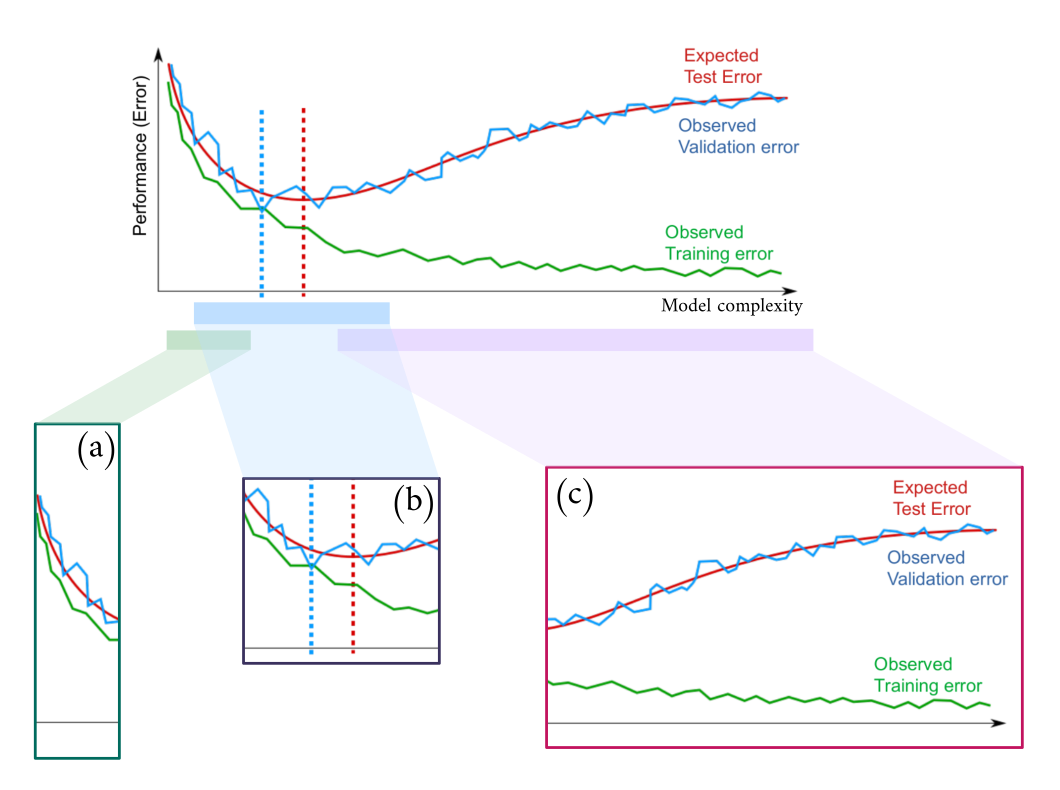
\includegraphics[width=0.8\textwidth]{ex_train_val_test.png}
% \end{figure}
\myFigure{Training versus validation exercise image}
{fig:ex-q1-training-vs-validation}
{ex_train_val_test.png}

\begin{itemize}
	\item[Q1.1] What is the whole figure about?
	\item[A1.1] ~\\
	      The Figure \ref{fig:ex-q1-training-vs-validation} shows the bias-variance tradeoff
	      for a model within the context of the regression problem.
	      The bias gives errors due to erroneous assumptions in the learning procedure.
	      In contrast, the variance yields errors due to the sensitivity of the model
	      to the training set fluctuations i.e. noise in the training dataset.
	      The three error lines displayed in the plot correspond to:
	      \begin{itemize}
		      \item Observed training error, from training set
		            used to fit the model on training data
		      \item Observed validation error, from test set assessing performance
		            meaning how well the model generalizes to unseen data
		      \item Expected test error, from an ideal unbiased dataset
		            assessing performance on unseen data
		            meaning how well the model would ideally generalize to unseen data
	      \end{itemize}

	      Along the x-axis, model complexity is intended as more hidden layers or neurons in the model.
	      In this particular model we can see that the observed training error
	      is decreasing as the model complexity increases, this will lead to overfitting.
	      Along the y-axis, the lower the performance metric, the better the model
	      since it measures the error of the model.

	\item[Q1.2] Explain the behaviours of the curves in each of the three highlighted sections in the figure, namely (a), (b), and (c).
	\item[A1.2] In Figure \ref{fig:ex-q1-training-vs-validation}:
	      \begin{itemize}
		      \item[a.] this is associated with the start of the training process,
		            when the model is \textit{underfitting} the data, has high bias and low variance.
		            The model is excessively simple to capture the underlying patterns from the dataset,
		            that is evident from the high observed training error,
		            and also the validation error is high as a consequence of the non-generalization of the model
		            with unseen data from the test set.
		            Test set and not validation set because there is no model selection process involved.
		            The model has high bias and low variance at start.
		            As the model complexity increases, the training error decreases
		            and the model starts to learn the patterns in the data.
		            However, the validation error also decreases at the beginning
		            but after a certain point starts to increase.

		      \item[b.] this window is associated optimal bias-variance tradeoff.
		            The ideal optimal model complexity $\theta^o$ references the red dotted vertical line,
		            and the optimal model complexity point according to the validation set $\theta_m$
		            references the blue dotted line.



		      \item[c.]
	      \end{itemize}

	      \begin{itemize}
		      \item[Q1.2.a] Can you identify any signs of overfitting or underfitting in the plot?
		            If yes, explain which sections correspond to which concept.
		      \item[A1.2.a] ~\\

		      \item[Q1.2.b] How can you determine the optimal complexity of the model based on the given plot?
		      \item[A1.2.b] ~\\
	      \end{itemize}

	\item[Q1.3] Is there any evidence of high approximation risk? Why?
	      If yes, in which of the below subfigures?
	\item[A1.3] ~\\

	\item[Q1.4] Do you think that increasing the model complexity can bring the training error to zero?
	      And the structural risk?
	\item[A1.4] ~\\

	\item[Q1.5] If the X axis represented the training iterations instead,
	      would you think that the training procedure that generated the figure used early stopping?
	      Explaib why. (\textbf{NB:} ignore the subfigures and the dashed vertical lines)
	\item[A1.5] ~\\

\end{itemize}

\subsection*{Q2. Linear Regression}
Comment and compare how the (a.) training error, (b.) test error and (c.) coefficients would change in the following cases:
\begin{itemize}
	\item[Q2.1] $x_3 = x_1 + 0.2 \cdot x_2$.
	\item[A2.1] ~\\

	\item[Q2.2] $x_3 = x_1 ** 2$ (in Python ** is the "power" operator, so  3 ** 2 = 3 * 3 = 9).
	\item[A2.2] ~\\

	\item[Q2.3] $x_3$ is a random variable independent from $y$.
	\item[A2.3] ~\\

	\item[Q2.3] How would your answers change if you were using Lasso Regression?
	\item[A2.3] ~\\

	\item[Q2.4] Explain the motivation behind Ridge and Lasso regression and their principal differences.
	\item[A2.4] ~\\
\end{itemize}

\subsection*{Q3. Logistic Regression}
\begin{itemize}
	\item[Q3.1] What are the main differences between the logistic-regression and the perceptron?
	\item[A3.1] ~\\

	\item[Q3.2] Discuss the major limit they share and how neural networks can solve it.
	\item[A3.2] ~\\

	\item[Q3.3] What is the role of activation functions in feedforward neural networks.
	\item[A3.3] ~\\
\end{itemize}

\subsection*{
	Q4. Consider the regression problem shown in the picture \ref{fig:ex-q4-regression}
	below and answer each point.
}

% \begin{figure}[htbp] %
% 	\centering
% 	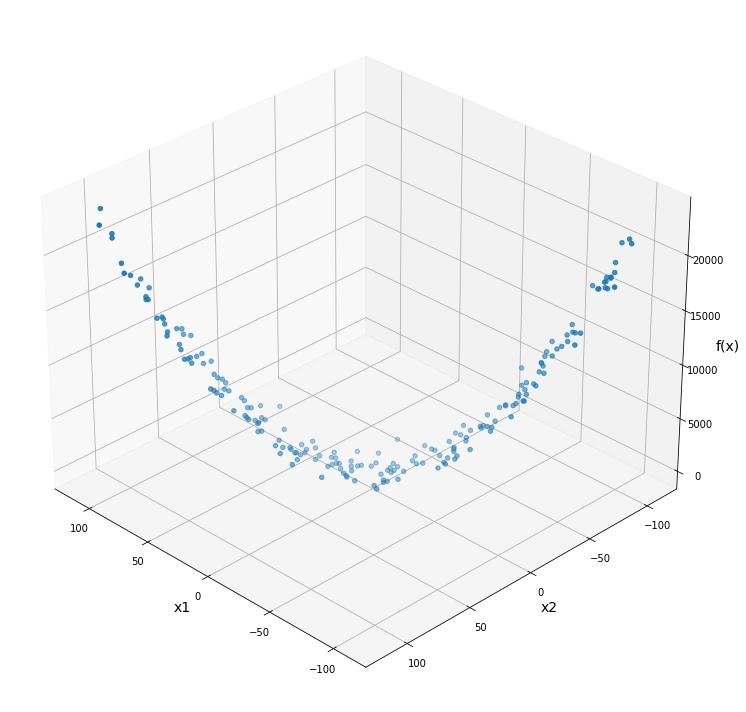
\includegraphics[width=0.7\textwidth]{figures/parabolic.jpg}
% \end{figure}
\myFigure{Regression problem}{fig:ex-q4-regression}{parabolic.jpg}

\begin{itemize}
	\item[Q4.1] Do you think a model of the family f(x, theta) = $\theta_0 + \theta_1 * x_1 + \theta_2 * x_2$ is a good choice for such task? Why?

	\item[A4.1] The simple linear model $f(x, \theta)$ would not be a good fit for the data.
	      It is evident that the data does not follow a linear trend.
	      The linear model would lead to underfitting where the model is not able
	      to capture the underlying patterns.
	      The relationship between the inputs variables
	      and the dependent output variable seems to be non-linear,
	      describing a quadratic interaction on both $x_1, x_2$ resulting in a parabolic shape.
	      A linear relationship among input variables as in $f(x, \theta)$
	      would not capture the curvature form of the data.

	\item[Q4.2] Do you think using a feed-forward neural network would improve the results?

	\item[A4.2] Using an FFNN would be a good choice for this problem task.
	      It is for sure better than the simple model with linear relationship
	      between independent input variable $x_1, x_2$
	      and dependent output variable $f(x, \theta)$.
	      In general, with FFNNs we can leverage the \textit{Universal Approximation Theorem (1991)}
	      which states that an FFNN with a single hidden layer containing a finite number of neurons
	      and a linear ouput neuron can approximate any continuous function
	      on compact subsets of $\mathbb{R}^n$.
	      Moreover, FFNN are highly flexible and can approximate virtually any function,
	      so complex non-linear relationship patterns,
	      which are hard for linear and polynomial regression,
	      are handled through the encapsulated abstraction of the neurons in the hidden layer(s).
	      In this case, the parabolic shape of the data would be captured,
	      as FFNN are a common choice for regression tasks with non-linear data.

\end{itemize}

\end{document}
